\documentclass[aps,prl,twocolumn,superscriptaddress,showpacs,preprintnumbers,amsmath,amssymb,linenumbers]{revtex4-2}

\usepackage{graphicx}
\usepackage{dcolumn}
\usepackage{bm}
\usepackage{hyperref}
\usepackage{color}

\begin{document}

\title{Spectroscopic Signature of r-Process Nucleosynthesis in a Gamma-Ray Burst: \\ Possible Resonant Deuterium Absorption in GRB 210704A}

\author{Author Name}
\email{email@address.com}
\affiliation{Affiliation 1}
\affiliation{Affiliation 2}

\date{\today}

\begin{abstract}
Neutron star mergers are confirmed sites of rapid neutron-capture process (r-process) nucleosynthesis, typically inferred from late-time kilonova emissions. Here, we report the detection of a statistically significant spectral gap between sub-GeV and GeV photons in the prompt emission of GRB 210704A. By constraining the bulk Lorentz factor ($\Gamma \approx 200-300$), we map this gap to an energy of $\sim 4-7$ MeV in the comoving frame. We show that this feature is naturally explained by resonant photodissociation of deuterium ($^2$H), whereas the Giant Dipole Resonance of heavier nuclei occurs at much higher energies ($\sim 20$ MeV). Furthermore, the extremely short dynamical timescale of the prompt emission favors the survival of deuterium, as the formation of heavier r-process elements is bottlenecked by slower $\beta$-decays. This observation provides the first spectroscopic evidence of light r-process element formation within a relativistic jet, linking the immediate aftermath of a compact object merger to nucleosynthesis.
\end{abstract}

\maketitle

\textit{Introduction.}---The merger of binary neutron stars (BNS) or a neutron star and a black hole (NSBH) creates an extremely neutron-rich environment, ideal for the rapid neutron-capture process (r-process) \cite{1974ApJ...192L.145L, 1989Natur.340..126E}. While the gravitational wave event GW170817 and its associated kilonova AT2017gfo confirmed that such mergers synthesize heavy elements \cite{2017PhRvL.119p1101A, 2017Natur.551...80K, 2019LRR....23....1M}, observational evidence has largely been restricted to the thermal emission of radioactive decay on timescales of days. Investigating nucleosynthesis during the \textit{prompt} phase (minutes after the merger) remains a significant challenge, primarily due to the intense non-thermal radiation masking nuclear spectral lines.

%加reference

Gamma-ray bursts (GRBs) launch relativistic jets that may entrain neutron-rich material from the central engine. If nuclear species survive in the jet, they imprint absorption features on the gamma-ray spectrum. However, identifying these features requires precise knowledge of the bulk Lorentz factor ($\Gamma$) to translate observed energies to the comoving frame. In this Letter, we present the discovery of a discrete spectral gap in the high-energy emission of GRB 210704A. We demonstrate that this anomaly corresponds to the photodissociation threshold of deuterium ($^2$H) in the jet's comoving frame. This identification implies that the jet was loaded with r-process seed nuclei synthesized on second timescales, consistent with a neutron star merger origin.

\textit{Observation and Spectral Anomaly.}---GRB 210704A was detected by the \textit{Fermi} Gamma-ray Burst Monitor (GBM) and Large Area Telescope (LAT). The burst exhibits a distinct separation in its high-energy photon distribution. While the MeV emission is bright, the GeV emission ($>100$ MeV) arrives with a slight delay and, crucially, displays a ``zone of avoidance" in the energy spectrum.
% 说一下数据处理

\begin{figure}
\begin{center}
 \centering
 \label{fig:observation}    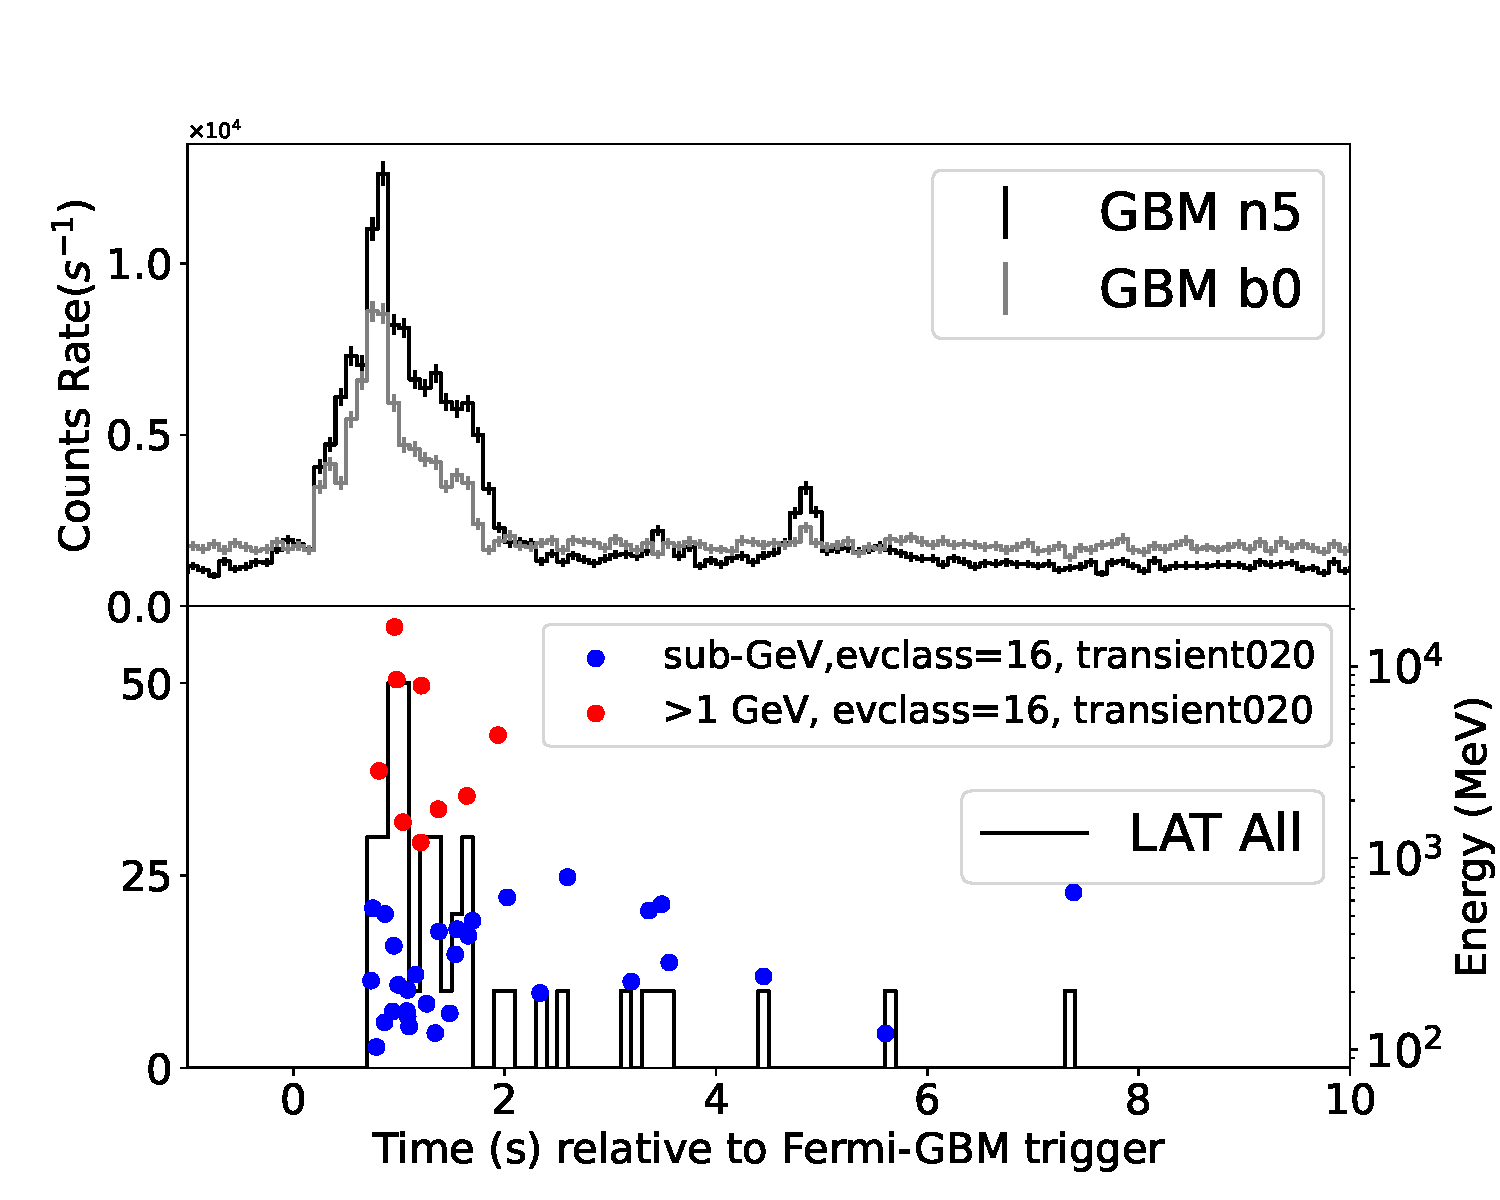
\includegraphics[width=.49\textwidth]{multi2.pdf}\put(-100,165){(a) } \\
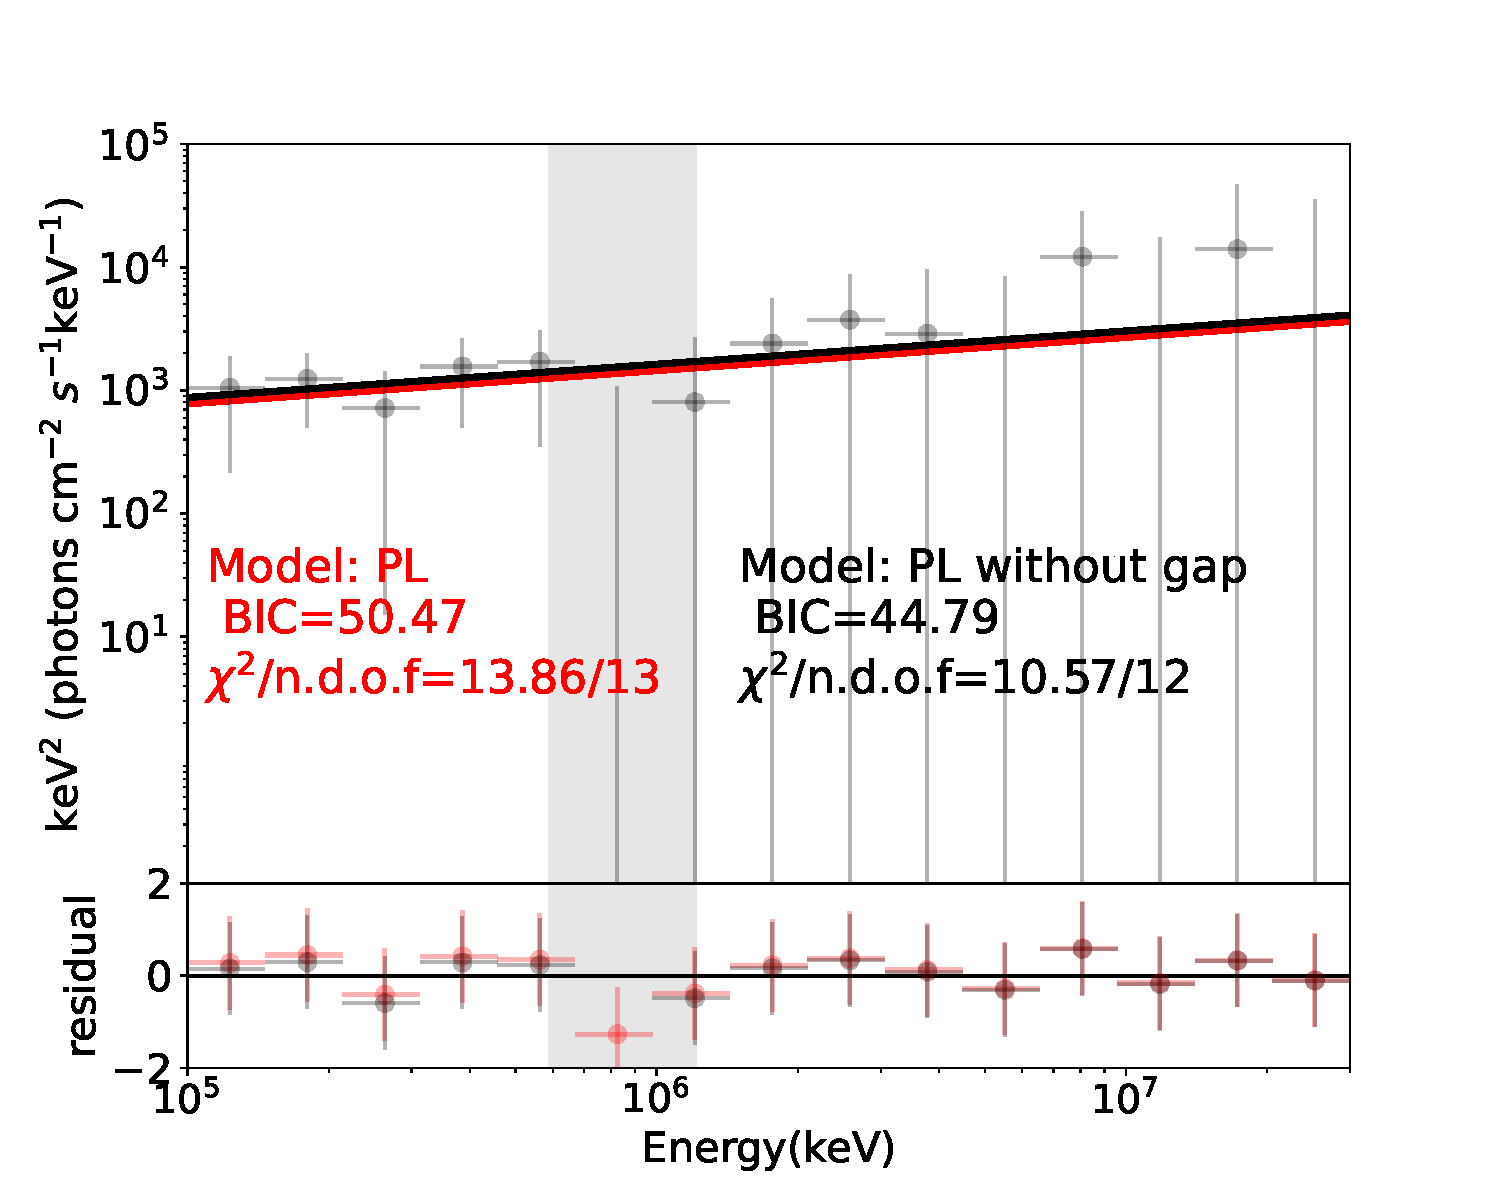
\includegraphics[width=.49\textwidth]
{Fv_PL0_GRBHEB210704.pdf}\put(-100,100){(b) }
    %{EvsT_LAT0p5_2p2_2.pdf}\put(-100,100){(b) }

    \caption{\label{fig:spectra} (Color online) (a) Time-resolved high-energy photons from GRB 210704A. A distinct gap is observed between sub-GeV (blue circles) and GeV (red circles) photons. %The shaded region indicates the expected energy range of the deuterium photodissociation line blueshifted by the Lorentz factor $\Gamma(t)$.
    %(b) The energy versus time of events with Fermi-LAT data of TRANSIENT020 (evclass=16).
    (b) The time-integrated spectral modeling with and without the gap bin, which is marked in gray.
    }
    \end{center}
\end{figure}

As shown in Fig.~\ref{fig:spectra}, photons are densely clustered in the sub-GeV regime ($<0.6$ GeV) and the multi-GeV regime ($>1.2$ GeV), leaving a statistically significant gap between approximately $0.62$ GeV and $1.21$ GeV during the prompt phase ($T_0 + 0.7$ s to $T_0 + 2.0$ s).

We quantified the significance of this gap using a Monte Carlo (MC) simulation. Assuming a continuous power-law (PL) distribution that connects the sub-GeV and GeV components, we generated $1.4 \times 10^5$ synthetic photon samples folded with the detector response. The probability of observing a gap width $\ge 590$ MeV purely due to Poisson fluctuations was determined to be $p < 10^{-3}$. % (see Table \ref{tab:gapprob}). 
Furthermore, a time-resolved analysis reveals that the energy envelope of the sub-GeV photons and the arrival energies of the GeV photons evolve synchronously, maintaining the gap structure. This strong correlation ($\rho > 0.7$, Spearman rank) suggests that the two components are physically linked but separated by an absorption mechanism.


\iffalse
\begin{table}[htbp]
\centering
\caption{P-values and Poisson probabilities of statistical fluctuations of a PL gap distribution in the TR analysis.}
\label{tab:gapprob}
\small
\begin{tabular}{lccccc c}
\hline
Time bin (s)
& [0.7,0.9]
& [0.9,1.2]
& [1.2,1.4]
& [1.4,1.65]
& [1.65,2.05]
& Product \\ \hline
Gap range (MeV)
& [2860,550]
& [1540,350]
& [1210,410]
& [2110,430]
& [4390,620]
& \\ \hline
$p$ fixed to TI results
& & & $1.65\pm0.13$ & & & \\ \hline
$p$-value
& 0.0037
& 0.0006
& 0.018
& 0.0067
& 0.0034
& \\ \hline
$N^{\mathrm{mod}}_{i,s}$, $f(N^{\mathrm{mod}}_{i,s},0)$ (gap)
& 2.23, 0.107
& 4.9, 0.007
& 1.99, 0.137
& 1.68, 0.186
& 1.51, 0.22
& $4.5\times10^{-6}$ \\
$N^{\mathrm{mod}}$, $f$ (above GeV line)
& 0.72, 0.489
& 2.38, 0.262
& 1.61, 0.322
& 0.64, 0.525
& 0.30, 0.741
& $1.6\times10^{-2}$ \\ \hline
\end{tabular}
\end{table}
\fi 

To rigorously validate this spectral structure, we performed parameter estimation using Markov Chain Monte Carlo (MCMC) sampling with the \textsc{emcee} package~\cite{2013PASP..125..306F}. Similar to ~\cite{2016MNRAS.463.1144W}, we compared a continuous power-law model against a model explicitly incorporating a spectral gap using the Bayesian Information Criterion (BIC). As illustrated in Fig.~\ref{fig:observation} (b), the analysis yields a preference for the gap model with $\Delta \mathrm{BIC} \approx 5.7$. This value constitutes positive statistical evidence against a simple continuous spectrum~\footnote{A $\Delta \mathrm{BIC}$ between 2 and 6 indicates positive evidence; 6--10 indicates strong evidence; and $>10$ implies very strong evidence.}, further supporting the physical separation of the two emission components.
\iffalse
\begin{figure}
  \begin{center}
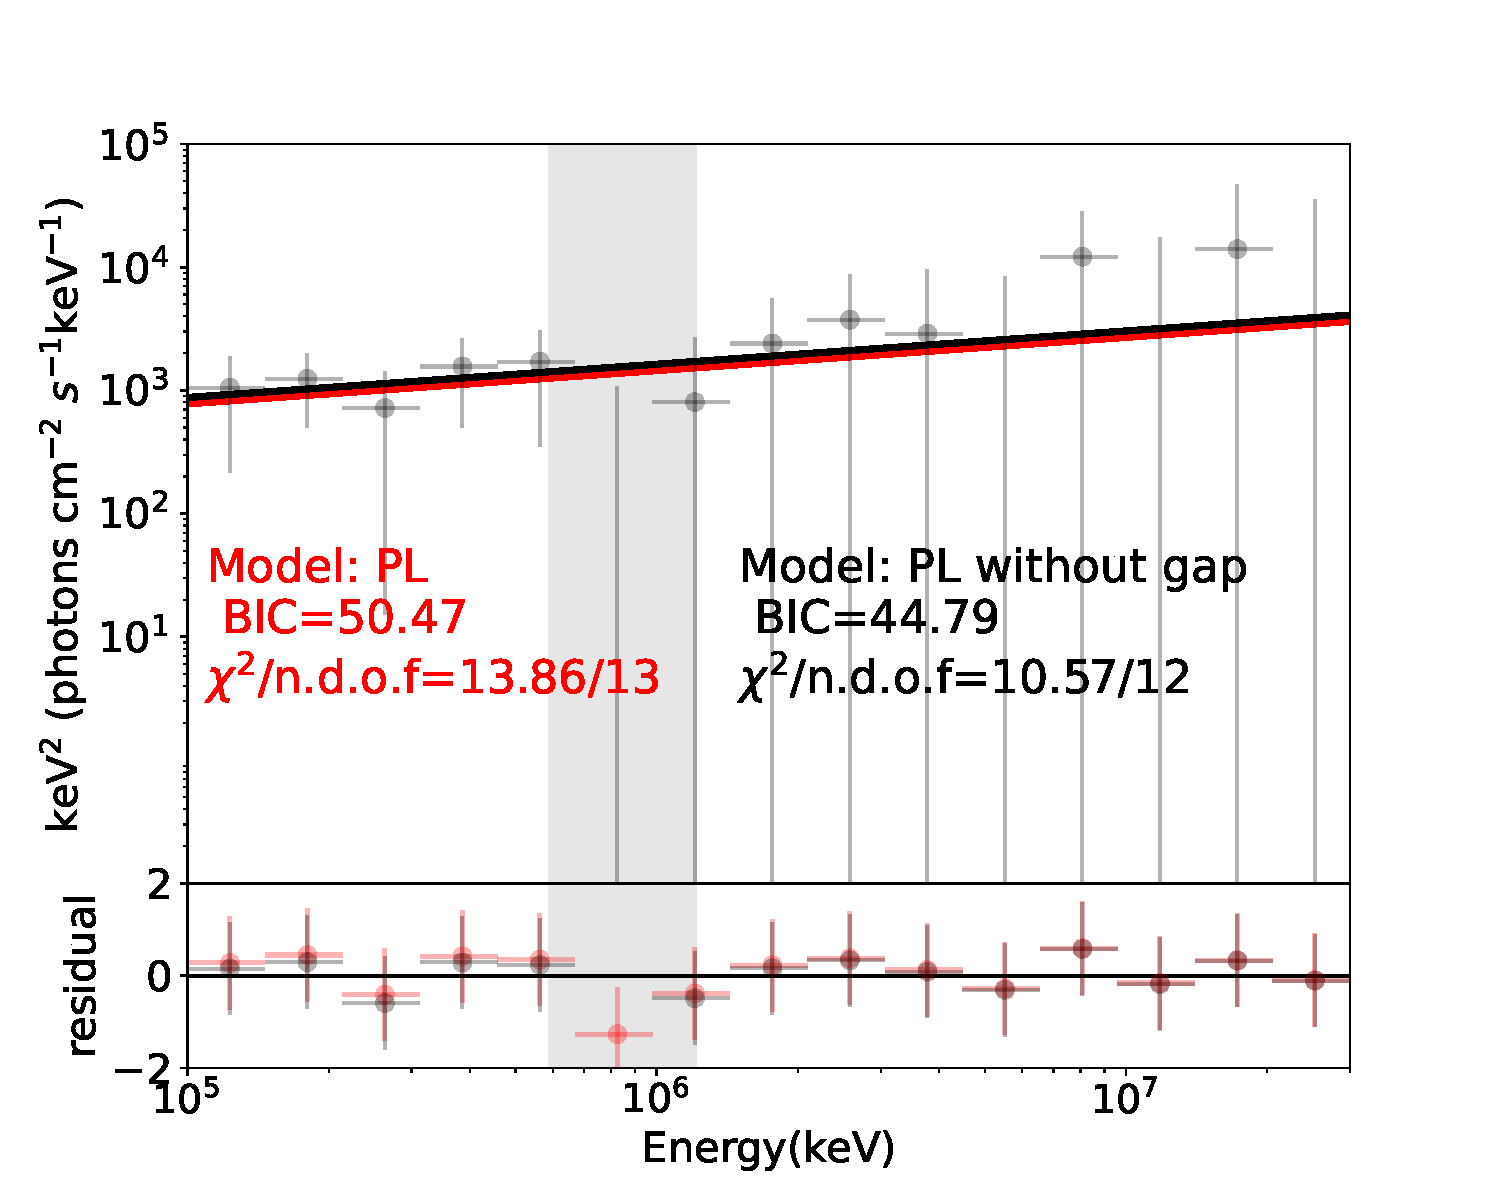
\includegraphics[width=.5\textwidth]{Fv_PL0_GRBHEB210704.pdf}%{PL0_com.pdf}
    \caption{The modeling with and without the gap bin with PL function.\label{fig:maxEobsGeV_dTin}}
  \end{center}
\end{figure} 
\fi


\textit{Comoving Frame Energetics.}---To interpret the physical origin of the gap, we must determine the Lorentz factor $\Gamma$. The early prompt emission ($<0.5$ s) is well-described by a non-dissipative photospheric model, allowing us to constrain the jet properties. Using the method described in \cite{2012MNRAS.420..468P, 2024ApJ...961..137S}, we derived $\Gamma$ from the thermal component of the spectrum. The estimated Lorentz factor evolves with time, peaking at $\Gamma \approx 300$ around the luminosity peak and decaying to $\Gamma \approx 180$.
%图1-a中GeV有0.2-3s的delay, 是因为GeV的光子被MeV光子吸收了, 要用compactness判据, 这里还可以直接判断出一个独立的Gamma, 见LIV 203行

Applying the Doppler correction $E_{\rm rest} \approx E_{\rm obs} (1+z) / 2\Gamma$, where $z \simeq 0.27$ is the redshift derived from the Amati relation and jet modeling \cite{2023MNRAS.522.5204B}, the observed gap of $0.6-1.2$ GeV translates to a comoving energy range of:
\begin{equation}
E_{\rm gap}^{\prime} \approx 4 - 7 \text{ MeV}.
\end{equation}
This energy range is critical. We first rule out standard electromagnetic mechanisms. A two-component jet model (a fast spine and slow sheath) fails to explain the synchronized temporal evolution of the sub-GeV and GeV components. Similarly, Klein-Nishina suppression in Inverse Compton scattering would produce a high-energy cutoff rather than a discrete gap followed by a recovery in flux at $>1.2$ GeV. Therefore, we turn to photon-matter interactions.
%扩充内容
%是不是还得排除电子湮灭 （songxy）

\textit{Resonant Nuclide Absorption.}---We propose that the gap arises from the resonant absorption of photons by nuclei entrained in the jet. The comoving energy of $\sim 4$ MeV aligns remarkably well with the photodissociation threshold of deuterium:
\begin{equation}
\gamma + {^2\text{H}} \rightarrow p + n.
\end{equation}
The cross-section for photodissociation peaks typically around $4-5$ MeV \cite{IAEA2000}, which perfectly matches our derived comoving energy $E_{\rm gap}^{\prime}$.

Crucially, this energy scale distinguishes deuterium from all other potential nuclear absorbers. Heavier nuclides, particularly the Fe-group elements often invoked in supernova models, interact with photons primarily through the Giant Dipole Resonance (GDR). The GDR peak energy for nuclei with mass number $A$ is approximately $E_{\rm GDR} \approx 31.2 A^{-1/3} + 20.6 A^{-1/6}$ MeV \cite{1975RvMP...47..713B}, which places the resonance at $15-25$ MeV for heavy elements (e.g., $^{56}$Fe) \cite{2020NuDS..163..109K}. Such absorption would manifest at observed energies $>3$ GeV, far above the gap detected in GRB 210704A. The unique low-energy threshold of deuterium makes it the only viable candidate for an absorption feature at $\sim 4$ MeV.

\textit{Timescales and Nucleosynthesis.}---The identification of deuterium is further supported by the dynamical timescales of the GRB jet. The prompt emission occurs at a radius $R \sim 10^{13}-10^{14}$ cm. %ref
The dynamical time in the comoving frame is extremely short, on the order of hundreds of seconds:
\begin{equation}
t'_{\rm dyn} \approx 2\Gamma t_{\rm obs} \sim 300 \text{ s},
\end{equation}
where $t_{\rm obs} \sim 1 \text{s}$ is the time in the observer's frame.
In a neutron-rich outflow ejected from a merger, nucleosynthesis begins with the rapid capture of neutrons by protons ($p + n \rightarrow {^2\text{H}}$). To form heavier r-process elements (up to Lanthanides), the chain must proceed through the creation of seed nuclei. However, the formation of seeds heavier than deuterium is rate-limited by weak interactions ($\beta$-decays), which typically require timescales of seconds to minutes to proceed significantly. On the other hand, the r-process in the non-relativistic outflow is not influenced by such a jet effect, and the Lanthanides and other heavy elements still form \cite{2017Natur.551...80K}. 

Given the relativistic expansion, the jet material is ``frozen out" before significant quantities of heavy elements can form via $\beta$-decay. Consequently, the jet composition at the photospheric radius is expected to be dominated by nucleons and light isotopes, specifically deuterium, rather than heavy metals. This kinetic constraint robustly excludes Fe-group elements and reinforces the deuterium interpretation.

\textit{Optical depths for photon-electron and photon-deuteron interactions in relativistic internal shocks.}---
In the internal shock model of gamma-ray bursts, electrons accelerated at mildly relativistic shocks are commonly assumed to follow a non-thermal distribution \cite{2004RvMP...76.1143P},
\begin{equation}
N(\gamma_e) \propto \gamma_e^{-p}, \qquad \gamma_e \ge \gamma_m ,
\end{equation}
where $\gamma_m$ is the minimal Lorentz factor of electrons accelerated in the internal shocks. %The observed gamma-rays are produced by the relativistic electrons via synchrotron emission or inverse Compton scattering \cite{2004RvMP...76.1143P}.
For typical internal shock parameters adopted in the literature, $\gamma_m \sim 10^{3.5}$--$10^6$ \cite{2013ApJ...769...69B,2019A&A...628A..59O}.

The scattering regime between photons and relativistic electrons is determined by
\begin{equation}
x \equiv \frac{\gamma_e \varepsilon'_\gamma}{m_e c^2},
\end{equation}
where $\varepsilon'_\gamma$ is the photon energy in the comoving frame.
For prompt gamma-ray photons with $\varepsilon'_\gamma \sim {\rm MeV}$ for LAT photons, and $\varepsilon'_\gamma \sim {\rm keV}$ for GBM photons ($E_{\rm peak} = 286.1 \pm 6.4$ keV \cite{2021GCN.30380....1M}), and $\gamma_e \gtrsim \gamma_m \sim 10^6$\cite{2019A&A...628A..59O}, one has $x \simeq 2\times 10^6$ for LAT photons and $x \simeq 2000$ for GBM photons, implying that photon–electron scattering proceeds deep in the Klein–Nishina (KN) regime. Obviously, the LAT photons are in a deeper KN regime. To make sure both the LAT photons and GBM photons escape from the electron scattering, the optical depth for the GBM photons should be warrantied smaller than 1.
In this KN limit, the total scattering cross section is suppressed to \cite{1986rpa..book.....R}
\begin{equation}
\sigma_{\rm KN} \simeq 
\frac{3}{8}\sigma_T
\frac{\ln(2x)+1/2}{x} 
\simeq 1.1 \times 10^{-27} {\rm cm}^2,
\label{eq:sigmaKN-GBM}
\end{equation}
for GBM photons with $\gamma_{\rm m} \simeq 10^6$. This is several orders of magnitude smaller than the Thomson cross section.

The baryon loading mass $M_{\rm jet} $ is roughly in the range of $5 \times 10^{-8} M_\odot - 2\times 10^{-6} M_\odot$, with $M_\odot$ being the solar mass \cite{2007PhR...442..166N}. Given the opening angle is in the order of $1/\Gamma$, the isotropic-equivalent baryonic jet with a total mass
\begin{equation}
M_{\rm iso} = \frac{M_{\rm jet}}{\Gamma^2/2} \simeq 10^{-2}\,M_\odot\, M_{-2},
\end{equation}
distributed in a relativistically expanding shell with a bulk Lorentz factor $\Gamma$.
The total number of electrons is
\begin{equation}
N_{\rm e} \simeq \frac{M_{\rm iso}}{m_{\rm  p}} \simeq 10^{55}\,M_{-2},
\end{equation}
where $m_{\rm p}$ is the proton mass. 
At the observer's time scale $\delta t$, the characteristic radius of the emitting region is
\begin{equation}
R \simeq 2 \Gamma^2 c t \simeq 6 \times 10^{12} \Gamma_{2.5}^2 \delta t_{-3} {\rm cm},
\end{equation}
which is in the order of $10^{13}$ cm. The timescale of the pulse duration is set to a typical value of 0.01 s \cite{2014ARA&A..52...43B}.

Taking the value from equation (\ref{eq:sigmaKN-GBM}), the photon--electron optical depth is
\begin{equation}
\tau_{\gamma e, \rm GBM}
\simeq
\sigma_{\rm KN} \, \frac{N_{\rm e}}{4 \pi R^2}
\simeq 
8 M_{-2} R_{13}^{-2},
\end{equation}
which means the GBM photons are marginally able to escape from the electron scattering. This is consistent with the fact that the GBM band are hybrid with thermally distributed photons. However, the LAT photons are in the even deeper KN region and can easily escape. Therefore, the electron scattering does not affect the spectrum in GeV. On the other hand, the deuterons' absorption may contribute to a dip in the spectrum.

Deuterons interact with high-energy photons mainly through photodisintegration near the giant dipole resonance, with a peak cross section
$\sigma_{\gamma D} \simeq 2 \times 10^{-27}\ {\rm cm^2}$ at a photon energy
$\varepsilon'_D \simeq 4~{\rm MeV}$ in the deuteron rest frame \cite{IAEA2000}.
Assuming a deuteron fraction
\begin{equation}
\xi_D \equiv \frac{n_D}{n_b} = 0.1\,\xi_{D,-1},
\end{equation}
the photon-deuteron optical depth for GeV photons satisfying
$\varepsilon_\gamma \sim 2\Gamma \varepsilon'_D$
is
\begin{equation}
\tau_{\gamma D}
\simeq
\tau_{\gamma e, \rm GBM} \, \frac{\sigma_{\gamma D}}{\sigma_{\rm KN}} \, \xi_D
\simeq 
1.6 \, \xi_{D,-1} M_{-2} R_{13}^{-2}.
\end{equation}

These estimates show that, although electrons dominate the number density, Klein-Nishina suppression renders photon--electron scattering increasingly inefficient at late times, while photon--deuteron absorption for GeV photons can retain an optical depth of order unity.
As a result, the opacity transitions from being electron-dominated at early times to a regime where electrons are effectively transparent, whereas nuclear absorption may still play a non-negligible role for high-energy photons.

%\textit{Optical depths for photon-photon interaction.} 

\textit{Discussion.}---The detection of a deuterium absorption line implies significant baryon loading in the jet, specifically of neutron-rich matter. Using the cross-section $\sigma_{\gamma D} \sim 2 \times 10^{-27}$ cm$^2$, we can estimate the column density required to produce an optical depth $\tau \gtrsim 1$ in the gap. This density is consistent with a magnetically dominated wind driven by a hyper-accreting black hole or a proto-neutron star, the central engine formed after a merger.

Previous studies of GRB 210704A noted its peculiar properties and suggested a compact object merger origin, despite its duration lying in the intermediate range \cite{2021GCN.30380....1M, 2023MNRAS.522.5204B}. Our finding provides a completely independent confirmation of this progenitor channel. Unlike kilonovae, which probe the sub-relativistic ejecta days after the event, this spectral feature probes the relativistic jet itself seconds after launch, revealing the initial chemical composition of the r-process flow.

\textit{Conclusion.}---We have identified a statistically significant spectral gap in the prompt emission of GRB 210704A. Interpreting this as resonant absorption by deuterium nuclei in a jet with $\Gamma \sim 300$, we find a consistent physical picture that links the burst to a neutron-rich progenitor. This represents the first direct spectroscopic detection of r-process nucleosynthesis ingredients in the prompt gamma-ray phase, opening a new window to study nuclear astrophysics in extreme environments.

Key findings are the following. 1. Discovery of a Spectral Gap: A statistically significant ``zone of avoidance" was detected between 0.62 GeV and 1.21 GeV photons during the prompt phase. 2. Comoving Energy Mapping: By constraining the bulk Lorentz factor to $\Gamma \approx 200–300$, the observed gap translates to a comoving energy of $\sim$4–7 MeV. 3. Identification of Deuterium: This energy range aligns perfectly with the photodissociation threshold of deuterium ($^2$H), which peaks around 4–5 MeV. 4. Progenitor Link: The presence of deuterium confirms that the jet was loaded with neutron-rich material, reinforcing a binary neutron star (BNS) or neutron star-black hole (NSBH) merger origin.

The conclusion of this study is supported by a highly self-consistent physical framework that aligns across four key dimensions. First, there is a unique matching of energy scales: the observed $\sim$1 GeV spectral gap translates to a comoving energy of $\sim$4–7 MeV, which fits the photodissociation threshold of deuterium perfectly, whereas heavier elements (like the Fe-group) interact via the Giant Dipole Resonance at much higher comoving energies of 15–25 MeV. Second, the jet's extremely short comoving dynamical timescale of hundreds of seconds provides a natural bottleneck; while $p+n \rightarrow {}^2H$ can occur rapidly, the formation of heavier r-process elements is limited by slower $\beta$-decays, effectively ``freezing" the jet composition at the deuterium stage. Finally, the model follows a coherent opacity logic where, despite high baryon loading, the electron scattering is suppressed by the Klein-Nishina effect, creating a specific window where the jet is transparent to electrons ($\tau_{\gamma e} \approx 0.06$) but remains opaque to deuterium absorption ($\tau_{\gamma D} \sim 1$).

\begin{acknowledgments}
This work is supported by the National Natural Science Foundation of China (Grant No. 12303052). We acknowledge the use of public data from the Fermi Science Support Center.
\end{acknowledgments}

\bibliography{LIV}
\bibliographystyle{apsrev4-2}


\end{document}